\documentclass[12pt]{article}

\usepackage{indentfirst}
\usepackage{hyperref}
\usepackage{graphicx}
\usepackage[margin=1in]{geometry}
\usepackage{setspace}

\usepackage[L7x,T1]{fontenc}
\usepackage[utf8]{inputenc}
\usepackage[lithuanian,english]{babel}

\graphicspath{ {./figures/} }

\setstretch{1.5}

\thispagestyle{empty}

\begin{document}
	\begin{center}

	    \vspace*{1cm}
	    \Large
	    Vilnius University

		Mathematics and Informatics Faculty

		Institute of Informatics 

		Bioinformatics study program
	    
        \vspace*{2cm}
        \Large
		\textbf{Protein thermostability prediction using 
		sequence representations from protein 
		language models}

	\end{center}

	\begin{flushright}

		\vspace*{2cm}
        \large
        Author: Ieva Pudžiuvelytė

        Supervisor: Kliment Olechnovič, PhD 
        
	\end{flushright}

	\begin{center}
		\vspace*{4cm}
        \large
        Course work project
        
        \vspace*{2cm}
        \large
        Vilnius, 2022
	\end{center}
	
	\newpage

	\tableofcontents

	\newpage
	
	\section{Introduction}

	This work is a prolongation of the previous work - the model 
	that performed binary classification into thermostability 
	classes. The model took ESM-1b protein embeddings as input 
	and provided prediction for each protein, how likely it 
	belongs to the thermostable class.
        
	\normalsize

	\newpage

	\section{Abstract in Lithuanian (Santrauka)}

	\begin{otherlanguage}{lithuanian}
		
	\end{otherlanguage}
	
	\newpage

	\section{Theory}

	\subsection{ESM-1b embeddings}

	\subsection{ProtTrans embeddings}

	\newpage

	\section{Methods}

	\subsection{Objective of this work}

	The main objective of this work is to analyse 
	which numerical representation of proteins is the most 
	suitable to use as input for the neural network 
	model to make binary protein classification into thermostability
	classes. Additionally, it was decided to try model 
	architectures with one or two hidden layers and evaluate 
	whether the different architecture improves the 
	performance.

	\subsection{Data set}

	The data set that was used for the research of this work was 
	used the same as for the training, validation, and testing of 
	the single-layer perceptron (SLP) with mean ESM-1b 
	representations in the previous work, although for this 
	research the data set was filtered out of identical sequences to 
	get more accurate evaluations.

	\begin{table}[h!]
		\caption{Number of sequences with embeddings before and after 
		filtering the data set}
		\vspace{0.2cm}
		\centering
		\begin{tabular}{ | c | c c | }
			\hline 
			Subset & Original & After filtering \\
			\hline 
			Training & 284309 & 283360 \\
			Validation & 65156 & 63158 \\
			Testing & 73662 & 73308 \\
			\hline    
		\end{tabular}
		\label{table:numberEmbeddings}
	\end{table}

	\begin{table}[h!]
		\caption{Number of sequences with embeddings in each class 
		before and after filtering the data set}
		\vspace{0.2cm}
		\centering
		\begin{tabular}{ | c | c c | }
			\hline 
			Class & Original & After filtering \\
			\hline 
			0 & 216595 & 212129 \\
			1 & 212729 & 207697 \\
			\hline    
		\end{tabular}
		\label{table:numberEmbeddingsClasses}
	\end{table}

	\newpage
	
	\subsection{Correlation analysis of embeddings' components}

	\begin{figure}[h!]
		\centering
		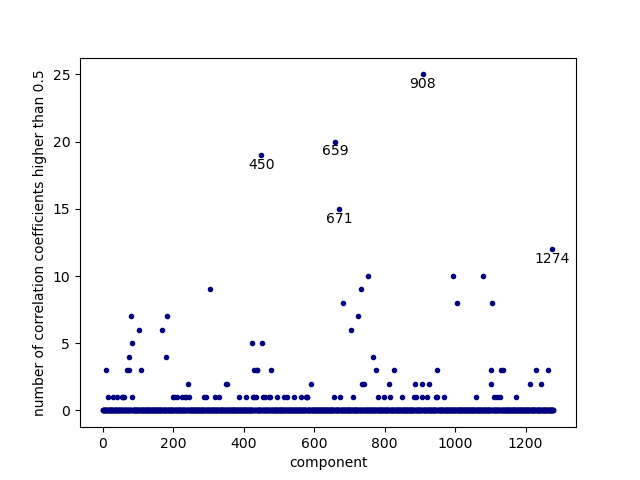
\includegraphics[scale=0.85]{validation_small_set_2_joined_correlation_high_corr.png}

		\caption{Plot of ESM-1b components that have got high correlation 
		coefficients with ProtTrans components}
		\label{figure:highCorrelationComponents}
	\end{figure}

	\newpage

	\begin{figure}[h!]
		\centering
		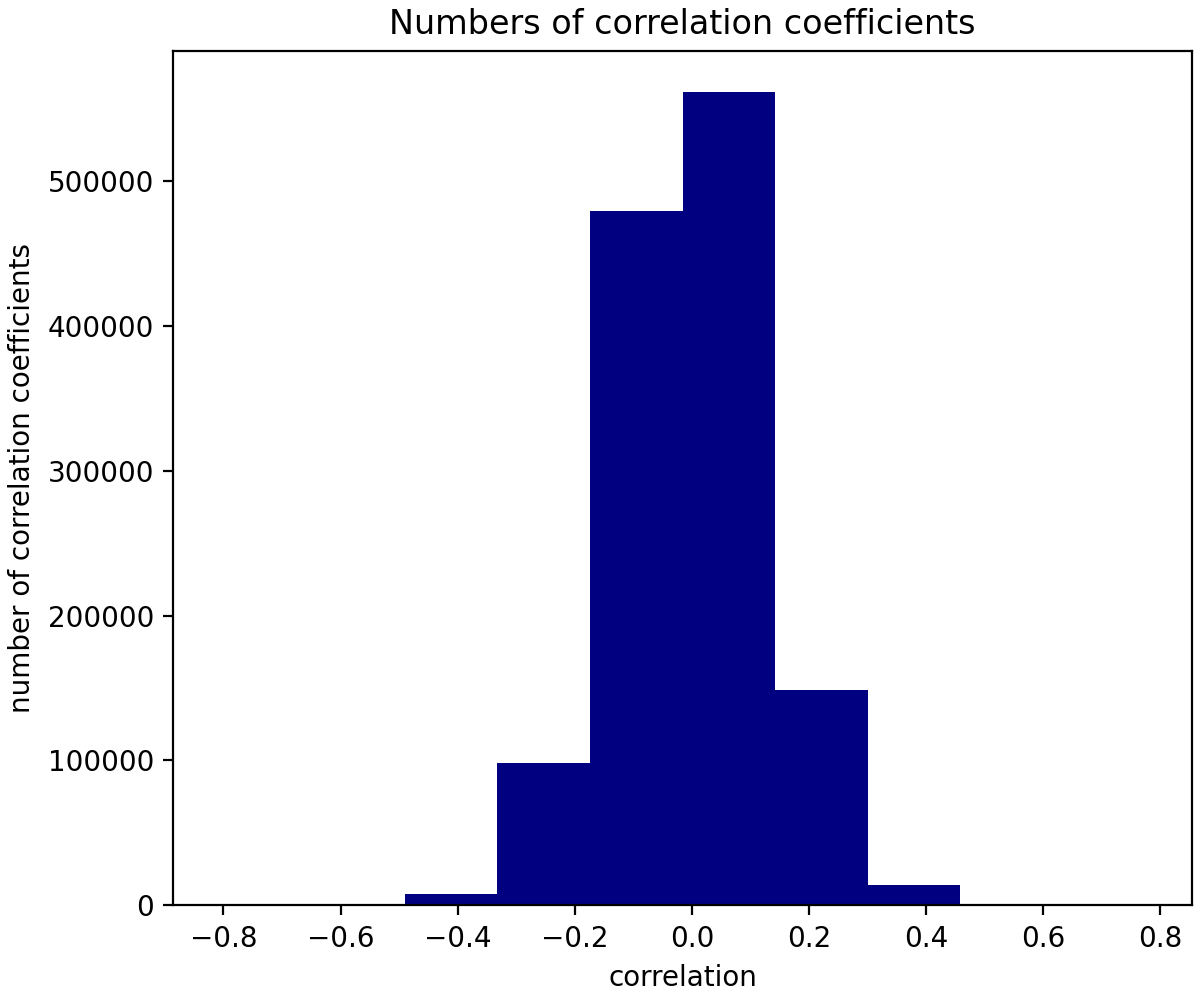
\includegraphics[scale=0.85]{validation_small_set_2_joined_correlation_hist.png}

		\caption{Histogram of correlation coefficients between ESM-1b 
		and ProtTrans components}
		\label{figure:correlationComponentsHisto}
	\end{figure}

	\newpage

	\begin{figure}[h!]
		\centering
		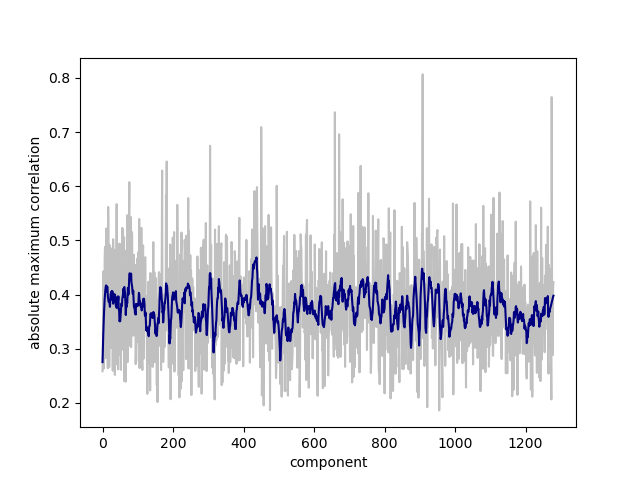
\includegraphics[scale=0.85]{validation_small_set_2_joined_correlation_max.png}

		\caption{Plot of ESM-1b components' maximum correlation coefficients with 
		ProtTrans components}
		\label{figure:correlationComponentsMax}
	\end{figure}

	\newpage

	\begin{figure}[h!]
		\centering
		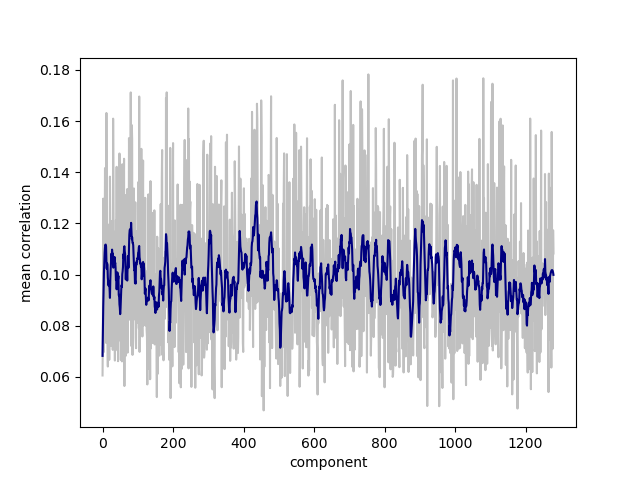
\includegraphics[scale=0.85]{validation_small_set_2_joined_correlation_mean.png}

		\caption{Plot of ESM-1b components' averaged  correlation coefficients 
		with ProtTrans components}
		\label{figure:correlationComponentsMean}
	\end{figure}

	\newpage

	\begin{figure}[h!]
		\centering
		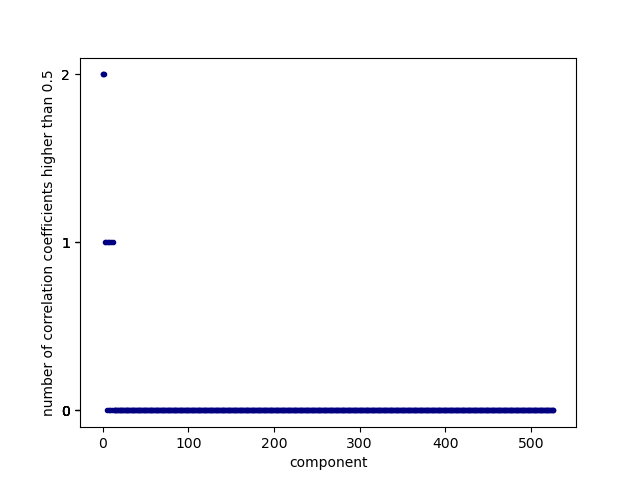
\includegraphics[scale=0.85]{validation_small_set_2_joined_PC_95_correlation_high_corr.png}

		\caption{Plot of ESM-1b principal components (explaining 
		95\% of data variation) that have got high correlation coefficients 
		with ProtTrans principal components (95\%)}
		\label{figure:highCorrelationComponentsPC95}
	\end{figure}

	\newpage

	\begin{figure}[h!]
		\centering
		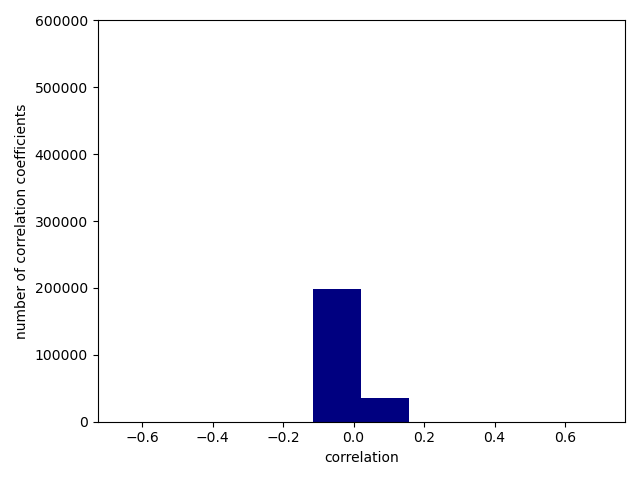
\includegraphics[scale=0.85]{validation_small_set_2_joined_PC_95_correlation_hist.png}

		\caption{Histogram of correlation coefficients between ESM-1b 
		and ProtTrans principal components (95\%)}
		\label{figure:correlationComponentsHistoPC95}
	\end{figure}

	\newpage

	\begin{figure}[h!]
		\centering
		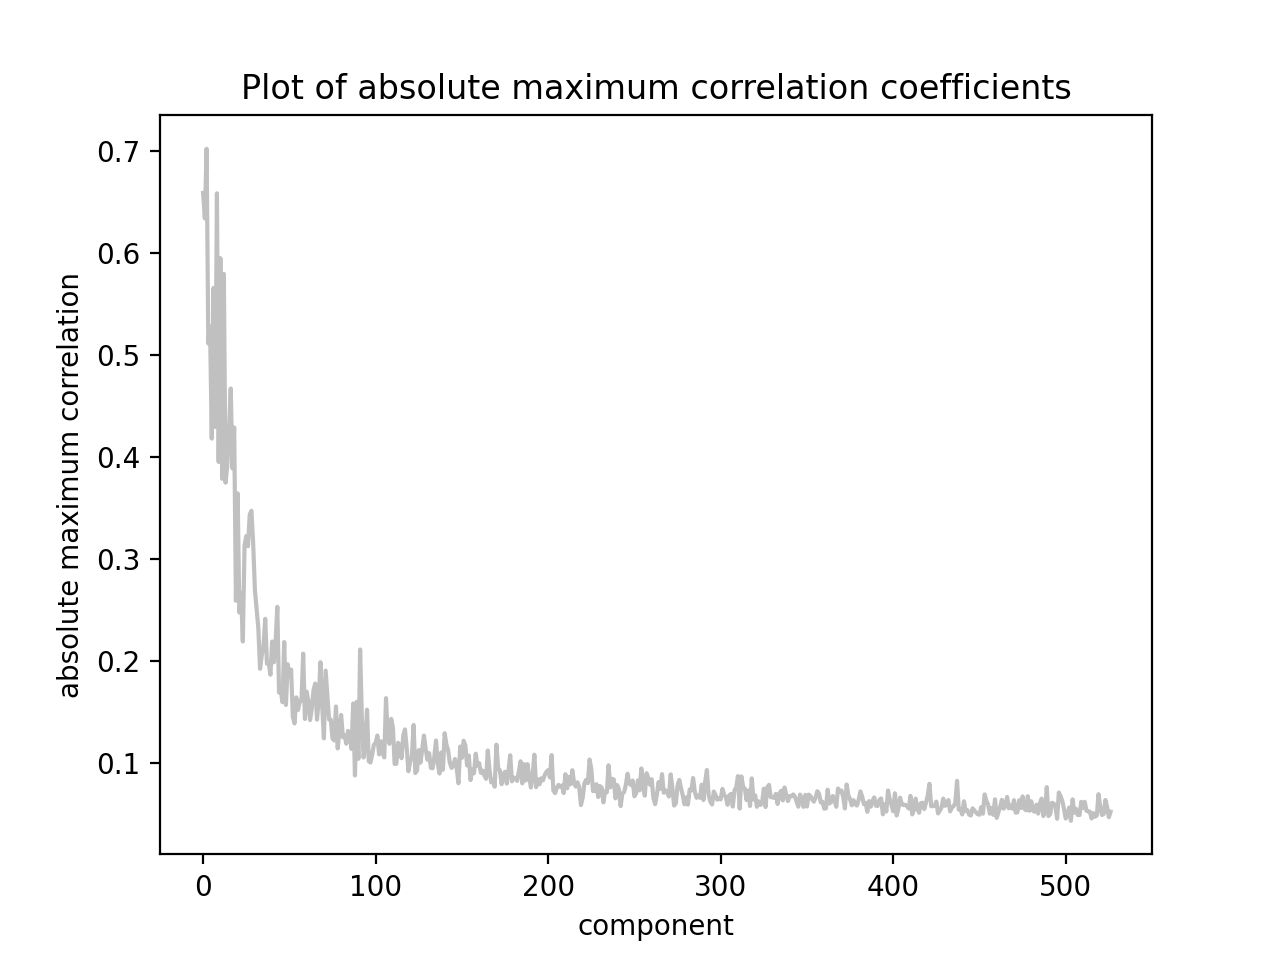
\includegraphics[scale=0.85]{validation_small_set_2_joined_PC_95_correlation_max.png}

		\caption{Plot of ESM-1b principal components' (95\%) maximum correlation 
		coefficients with ProtTrans principal components (95\%)}
		\label{figure:correlationComponentsMaxPC95}
	\end{figure}

	\newpage

	\begin{figure}[h!]
		\centering
		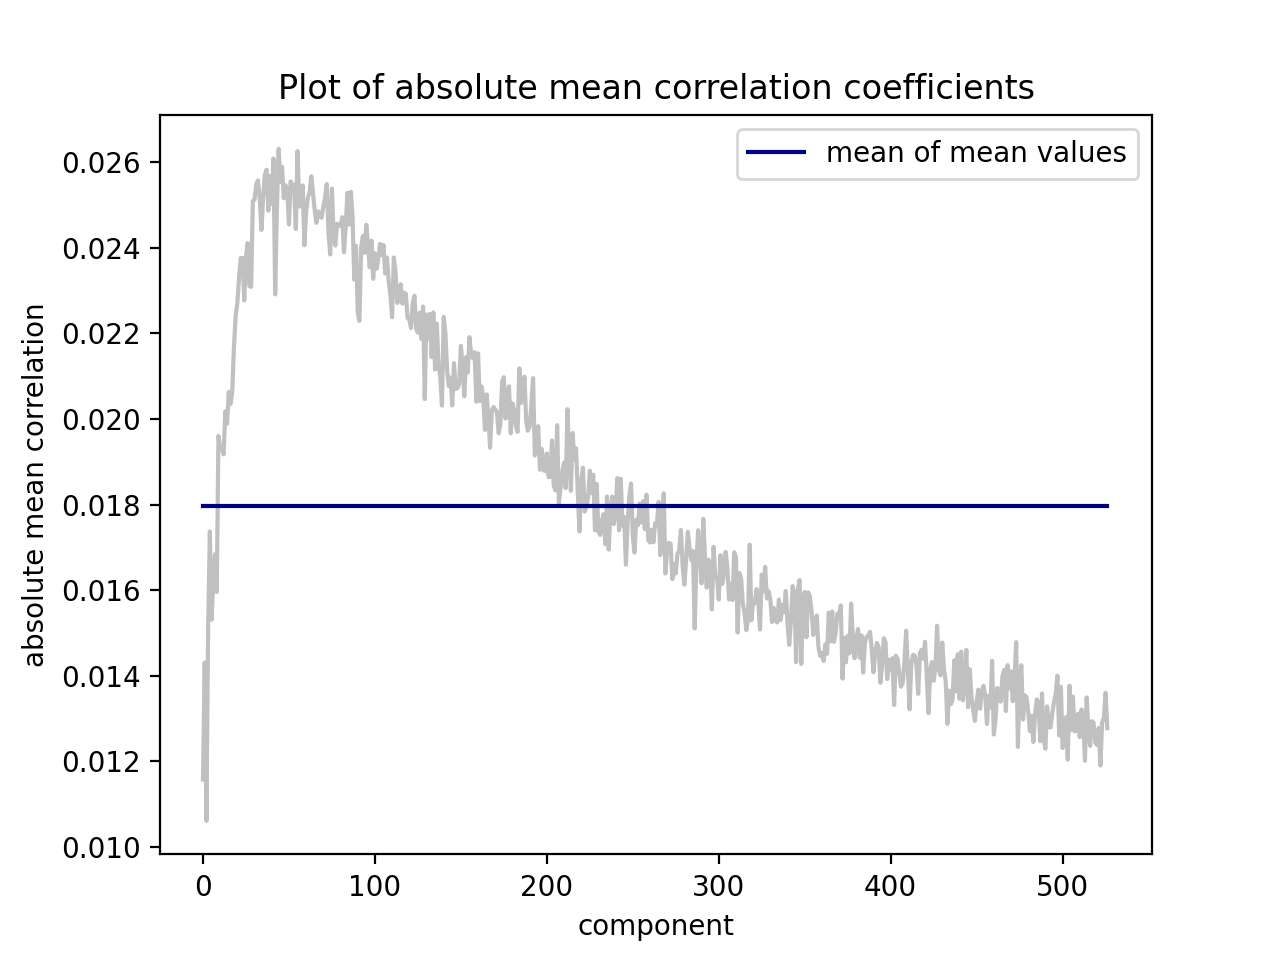
\includegraphics[scale=0.85]{validation_small_set_2_joined_PC_95_correlation_mean.png}

		\caption{Plot of ESM-1b principal components' (95\%) averaged correlation 
		coefficients with ProtTrans principal components (95\%)}
		\label{figure:correlationComponentsMeanPC95}
	\end{figure}

	\newpage

	\subsection{Analysed representations}
	
	Both protein language models - ESM-1b and ProtTrans - provide 
	per token or per residue representations - each 
	amino acid of the protein gets 1280 or 1024-dimensional vector from
	ESM-1b or ProtTrans model respectively. Therefore, each protein is 
	originally represented by ${m \times n}$ matrix, 
	where ${m}$ is the number of dimensions of the chosen type of embedding
	and ${n}$ is the number of amino acids that compose the protein. 
	These representations were processed to get vectors of the same dimension 
	for each protein in the data set. The representations 
	that were included in the analysis:

	\begin{enumerate}
		\item Mean ESM-1b and ProtTrans 
		\item Joined mean ESM-1b and ProtTrans
		\item Normalised mean ESM-1b and ProtTrans
		\item Joined normalised mean ESM-1b and ProtTrans
		\item Median ESM-1b and ProtTrans
		\item Minimum, median, and maximum ESM-1b and ProtTrans
		\item Quantiles (including minimum and maximum) ESM-1b and ProtTrans
		\item Quantiles (including minimum and maximum) and mean ESM-1b and ProtTrans
		\item Octiles (including minimum and maximum) ESM-1b and ProtTrans
	\end{enumerate}

	\begin{table}[h!]
		\caption{Sizes of the analysed representations' vectors}
		\vspace{0.2cm}
		\centering
		\begin{tabular}{ | c | c c | }
			\hline 
			Representation & ESM-1b & ProtTrans \\
			\hline 
			Mean & 1280 & 1024 \\
			Joined mean & \multicolumn{2}{c|}{2304} \\
			Median & 1280 & 1024 \\
			Minimum, median, maximum & 3840 & 3072 \\
			Quantiles & 6400 & 5120 \\
			Quantiles and mean & 7680 & 6144 \\
			Octiles & 11520 & 9216 \\
			\hline    
		\end{tabular}
		\label{table:vectorsDimensions}
	\end{table}

	\newpage

	\subsection{Analysed architectures}

	\begin{table}[h!]
		\caption{Models that were tested with ESM-1b embeddings input}
		\vspace{0.2cm}
		\centering
		\begin{tabular}{ | c | c c | }
			\hline 
			Model & Number of hidden layers & Size of hidden layers \\
			\hline 
			C2H2\_h640-320 & 2 & 640, 320 \\
			C2H2\_h320-160 & 2 & 320, 160 \\
			C2H1\_h640 & 1 & 640 \\
			C2H1\_h320 & 1 & 320 \\
			C2H1\_h160 & 1 & 160 \\
			SLP\_ESM-1b & 0 & - \\
			\hline    
		\end{tabular}
		\label{table:modelArchitecturesESM}
	\end{table}

	\begin{table}[h!]
		\caption{Models that were tested with ProtTrans embeddings input}
		\vspace{0.2cm}
		\centering
		\begin{tabular}{ | c | c c | }
			\hline 
			Model & Number of hidden layers & Size of hidden layers \\
			\hline 
			C2H2\_h512-256 & 2 & 512, 256 \\
			C2H2\_h256-128 & 2 & 256, 128 \\
			C2H1\_h512 & 1 & 512 \\
			C2H1\_h256 & 1 & 256 \\
			C2H1\_h128 & 1 & 128 \\
			SLP\_ProtTrans & 0 & - \\
			\hline    
		\end{tabular}
		\label{table:modelArchitecturesPT}
	\end{table}

	\newpage

	\section{Results}

	\subsection{Representation analysis}

	\begin{figure}[h!]
		\centering
		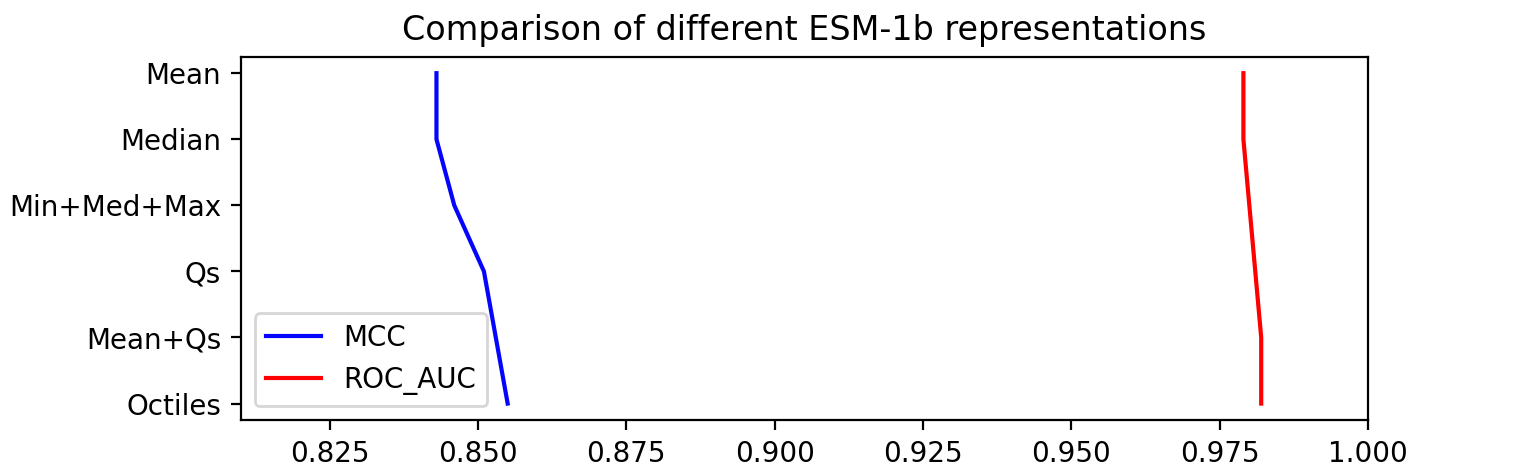
\includegraphics[scale=0.7]{SLP_ESM_003_diff_representations.png}

		\caption{Comparison of SLP models', which were trained with different
		ESM-1b representations, MCC and ROC AUC scores}
		\label{figure:scoresRepresentationsESM}
	\end{figure}

	\begin{figure}[h!]
		\centering
		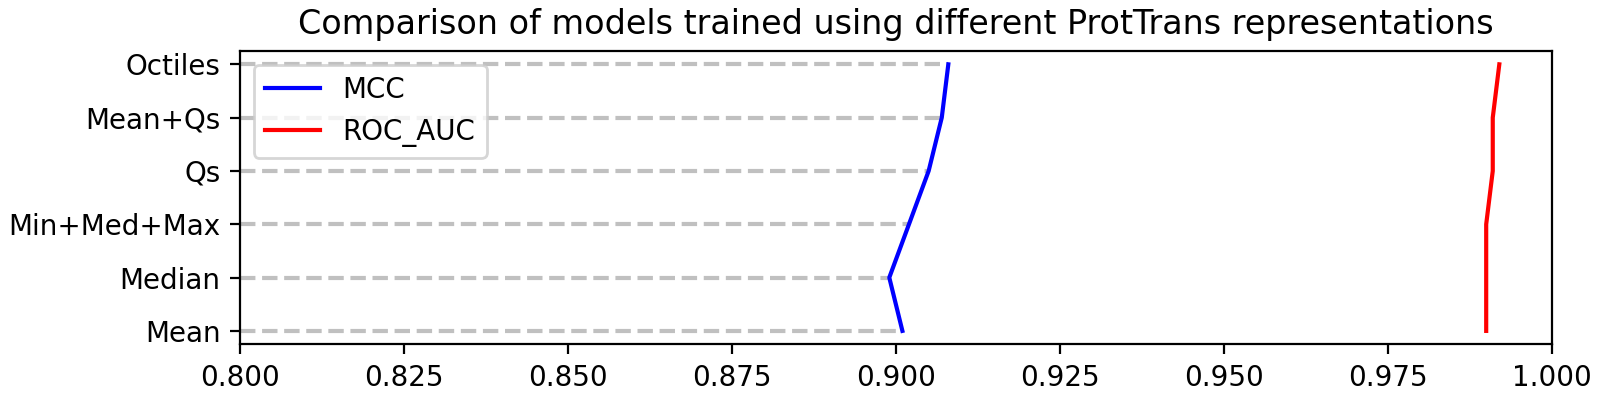
\includegraphics[scale=0.7]{SLP_PT_003_diff_representations.png}

		\caption{Comparison of SLP models', which were trained with different
		ProtTrans representations, MCC and ROC AUC scores}
		\label{figure:scoresRepresentationsPT}
	\end{figure}

	\newpage

	\subsection{Architecture analysis}

	\begin{figure}[h!]
		\centering
		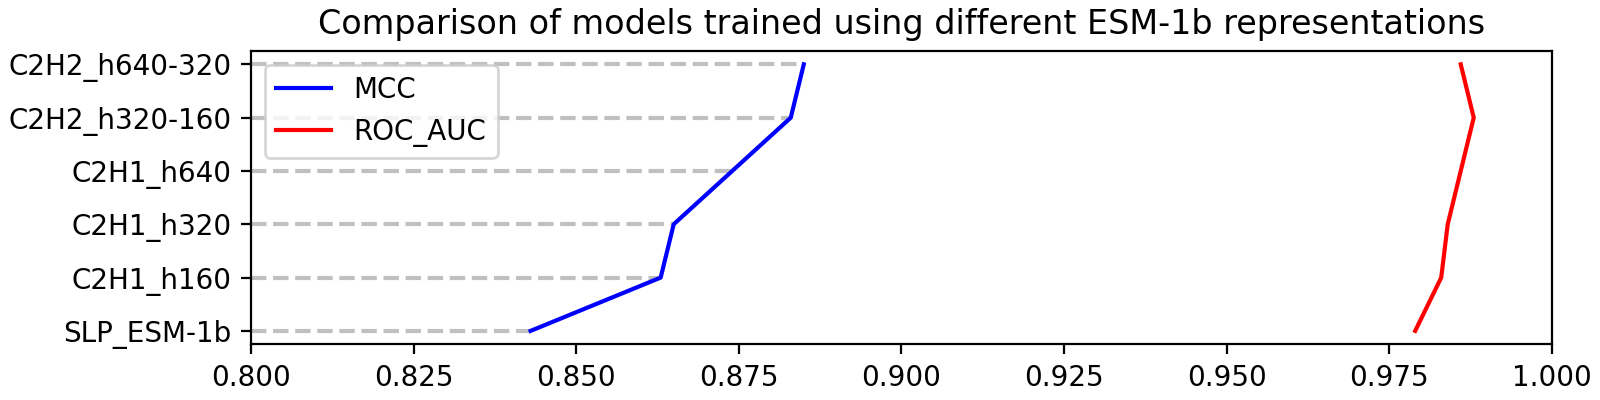
\includegraphics[scale=0.6]{MLP_ESM.png}

		\caption{Comparison of models', which were trained using 
		ESM-1b embeddings, MCC and ROC AUC scores}
		\label{figure:scoresMLP_ESM}
	\end{figure}

	\begin{figure}[h!]
		\centering
		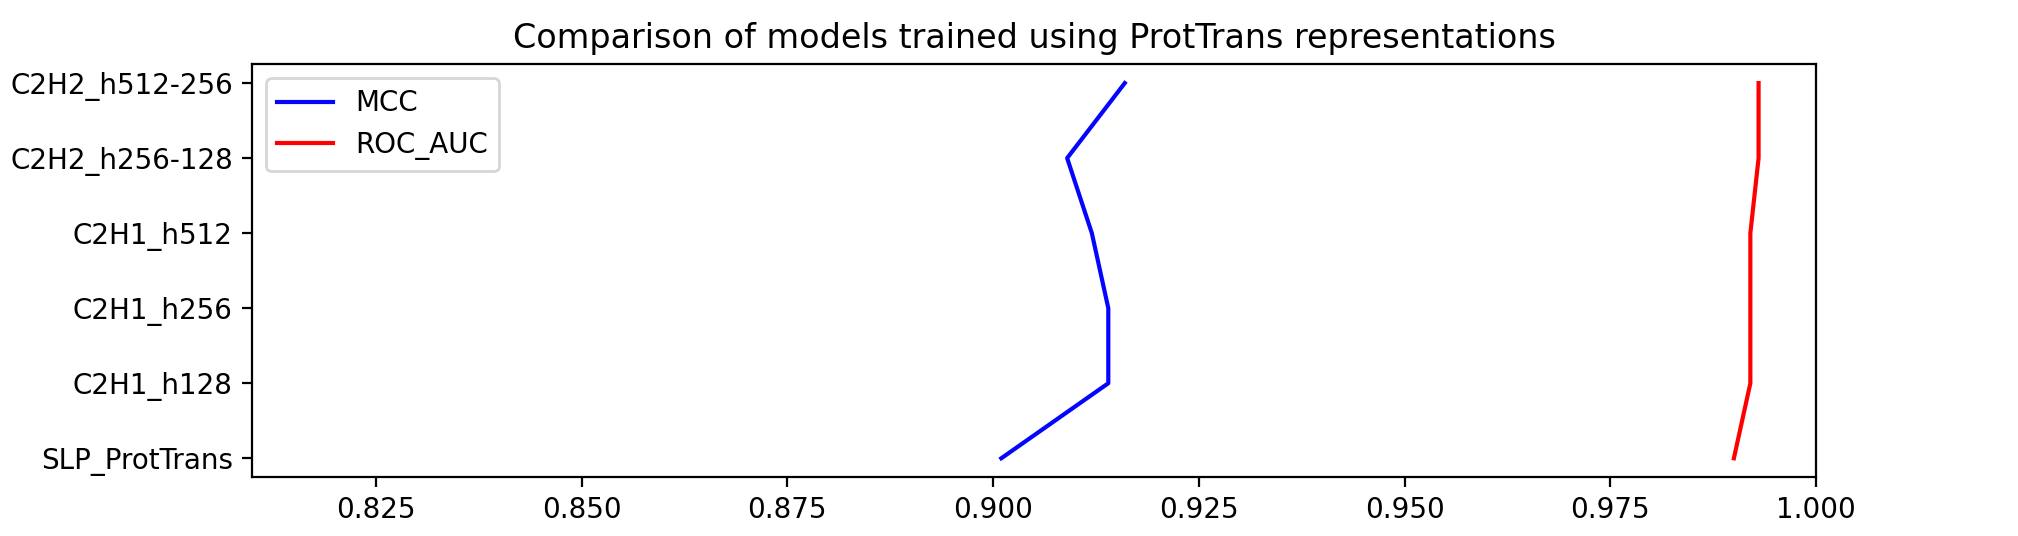
\includegraphics[scale=0.6]{MLP_PT.png}

		\caption{Comparison of models', which were trained using 
		ProtTrans embeddings, MCC and ROC AUC scores}
		\label{figure:scoresMLP_PT}
	\end{figure}

	\newpage

	\section{Conclusions}

	\newpage

	\section{Availability}

	The code that was used to receive the results of this work can be found
	in the designated Github repository: 
	\href{https://github.com/ievapudz/Course_Work_Project}{https://github.com/ievapudz/Course\_Work\_Project}.

	\newpage
	
	\nocite{*}
	
	\normalsize

\bibliography{references} 
\bibliographystyle{ieeetr}

\end{document}
